%%%%%%%%%%%%%%%%%%%%%%
\chapter{Equilibrium interface dynamics}
%%%%%%%%%%%%%%%%%%%%%%

%%%%%%%%%%%%%%%%%%%%%%
    \section{Introduction}
%%%%%%%%%%%%%%%%%%%%%%

Dans ce chapitre nous analysons la dynamique des systèmes statistiques. L'analyse nous permettra de comprendre comment les transitions de phase, notament certains systèmes subissant une séparation de phase à la transition, se comportent de manière dynamique. L'exemple le plus connu est le modèle d'Ising en absence de champ magnétique, le paramètre d'ordre de la transition étant la magnétisation totale du système. Dans la phase haute température, le système est homogène et sa magnétisation est nulle. En dessous de la température critique, dans le cas où le paramètre d'ordre est conservé (par exemple une dynamique de Kawasaki ou modèle B), le système va localement se séparer en deux phases de magnétisation moyenne opposée séparées par une interface minimisant l'énergie de surface entre les deux phases. 

Dans le cas où le paramètre d'ordre n'est pas conservé (par exemple une dynamique de Glauber ou modèle A), une brisure spontannée de symmétrie fera que l'une des deux phases englobe l'autre, au point de recouvrir tout le système (voir Fig \ref{clusterization}). Dans une transition de phase continue où le point critique est atteint depuis l'état désordonné vers l'état ordonné, les domaines de phase égales sont de taille égale à la longueur de corrélation du système. Dans les transitions de phase telles que celles du modèle d'Ising, cette longueur de corrélation diverge lorsque l'on s'approche de la température critique $T_C$. Dans un système thermodnamique, elle devient infinie, impliquant que le système prend un temps infini pour atteindre l'équilibre thermodynamique : c'est le ralentissement critique. Ce processus de croissance des domaines depuis la phase désordonnée s'appelle le \textit{coarsening} et la théorie de la cinétique d'ordre des phases est la théorie développée pour le comprendre.
Cette thèse s'appuie sur cette théorie afin de déterminer les propriétés statistiques (telles que la position moyenne et la tension superficielle) des interfaces entre deux phases coexistantes.
\begin{figure}[t]
    \centering
    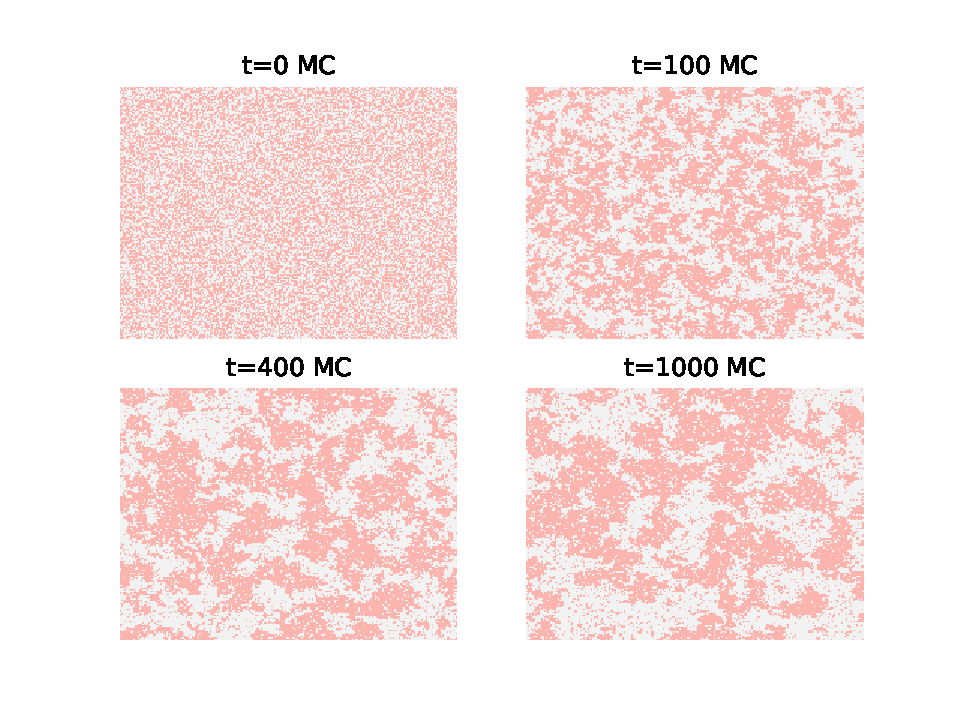
\includegraphics[width=0.9\linewidth]{intro/clusterization.pdf}
    \caption{Phénomène d'aggrégation à partir d'une trempe (\textit{quench}) dans un modèle d'Ising de $T=\infty$ à $T=T_{2D,C}$ \cite{onsager_crystal_1944} pour différents temps en étapes de Monte Carlo, pour un système $600 \times 600$ avec une dynamique non-conservée de Glauber.}
    \label{clusterization}
\end{figure}
$\bx$

In this chapter we will analyse the dynamics of statistical systems. The analysis will allow us to understand how phase transitions occur dynamically. For instance we know that certain systems undergo what is known phase separation, for instance if we take the Ising model with zero magnetic field, in the high temperature phase the system is homogeneous and the average magnetisation, which is the order parameter for the transition is zero. Below the critical temperature if the overall magnetisation is conserved (for instance for Kawasaki dynamics), which would be the case if spins corresponded to different types of particles, the system will separate into two  phases of opposite average magnetisation, separated by an interface which will be roughly flat in order to minimise the surface energy between the two phases. For nonconserved systems, where the overall magnetisation in not conserved (for example Glauber dynamics), eventually one of the two phases will make up the system (spontaneous symmetry breaking). In a continuous phase transition as the critical point is reached from the disordered to ordered, domains of phases of positive and negative magnetisation form and the size of these domains is given by the correlation length of the system. For continuous phase transitions such as that in the Ising model the correlation length diverges as as the critical point is approached, for instance as $T\to T_c$ if the temperature is varied. The size of the domains thus have to become infinite if the system is infinite, this means that for an infinite system it will take an infinite time to relax to the equilibrium state. The process of domain growth is known as coarsening and phase ordering kinetics is the theory that has been developed to understand the phenomenon of coarsening. Furthermore, for systems with a conserved order parameter which separate into two phases, the two phases will be separated by an interface. This interface will be characterised by a surface tension, its average position will be fixed but it will exhibit fluctuations. Later we will see how model of phase ordering kinetics and be used to determine the static and dynamical properties of interfaces between two coexisiting phases. 

While the phase diagram of a system can be determined via 
its Hamiltonian and equilibrium statistical mechanics, the dynamics of coarsening depends on details of the systems dynamics that do not show up in single time thermodynamic observables. Therefore one needs to construct dynamical models that capture the underlying evolution of the state of the system, in particular there is a big difference between systems where the order parameter is conserved and those where it is not conserved.

%%%%%%%%%%%%%%%%%%%%%%
    \section{Statics of systems with a finite number of degrees of freedom}
%%%%%%%%%%%%%%%%%%%%%%

Thermodynamic systems are naturally described in terms of fields, for example densities. This means that one is naturally lead to consider statistical field theories where the system is described in terms of a local field $\phi(\bx)$. Statistical field theories can be applied to both statics, to understand phase diagrams, and dynamics to understand phase ordering. However to start with we will examine the case of systems with a finite number of degrees of freedom. 

Consider a system in the canonical ensemble with a Hamiltonian $H(\bq)$ where $q_i$ for 
$1\leq i\leq N$ represent a finite number of continuous spatial degrees of freedom and where in a classical system we have already integrated over the corresponding momenta. The partition function for the system is given by
\begin{equation}
    Z = \int d\bq \exp\left(-\beta H(\bq)\right),
\end{equation}
and in equilibrium the probability density function $P_{eq}(\bq)$ of the degrees of freedom is given by 
\begin{equation}
    P_{eq}(\bq) = \frac{\exp\left(-\beta H(\bq)\right)}{Z}.\label{eqdis}
\end{equation}
In general the integral which gives the  partition function cannot be computed analytically.
The simplest approximation to compute $Z$ is the mean field approximation where the integral 
is approximated by the integrand at its largest value - in mathematics this is the Laplace method for approximating an integral and in this context it is just an expansion about the minimum energy configuration of the system. The mean field approximation is thus
\begin{equation}
    Z_{MF}= \exp\left(-\beta H(\bq^*)\right),
\end{equation}
where $\bq^*$ is the value of $\bq$ which minimises $H$ (note that the approximation becomes exact in the zero temperature limit - $\beta \to \infty$   - as the system will minimise its energy). The values $q_i^*$ are determined from
\begin{equation}
    \frac{\partial H}{\partial q_i}|_{\bq={\bf q^*}}=0.
\end{equation}
Within this approximation any thermodynamic observable is given by
\begin{equation}
    < f(\bq) > = f(\bq^*).
\end{equation}

We now consider how one can model dynamics of such systems. We will look for a Langevin equation which is chosen to give the correct equilibrium Gibbs-Boltzmann distribution. We write
\begin{equation}
    \frac{d q_i}{dt} = -L_{ij}\frac{\partial H(\bq)}{ \partial q_j} + \eta_i(t),
\end{equation}
where $L_{ij}$ is a matrix which discuss later and $\eta_i(t)$ is zero mean Gaussian white noise  with correlation function 
\begin{equation}
    < \eta_i(t)\eta_j(t')> =  \Gamma_{ij} \delta(t-t')\label{cfn}
\end{equation}
The Gaussian white noise represents the effects of thermal fluctuations on the system we assume that the correlation time of these fluctuations is extremely short with respect to the dynamics of the degrees of freedom $q_i$ (in fact in critical systems the dynamics becomes very slow, critical slowing down, and this approximation becomes better and better as one approaches the critical point).  There is no momentum term in this Langevin equation and for this reason it is often called the over damped Langevin equation. Overdamped Langevin equations can also be derived staring from Newton's laws in the presence of friction, due to a solvent, and again white noise (again due to molecular collisions with the solvent) and by taking the limit where the frictional forces are greater than the acceleration term in Newton's equations (equivalent to setting the particle masses to zero).


As Eq. (\ref{cfn}) is for a correlation function the matrix $\Gamma_{ij}$ must be symmetric and cannot have any negative eigenvalues.

In the absence of noise or thermal fluctuations, so at zero temperature, the system will simply minimise its energy. Therefore if 
\begin{equation}
    \frac{\partial H(\bq)}{ \partial q_j} =0, 
\end{equation}
with no noise we have $\frac{d q_i}{dt}=0$, that is to say it is the term $\frac{\partial H(\bq)}{ \partial q_j}$ that drives the dynamics if there is no noise. As long as the matrix $L_{ij}^{-1}$ exists the zero temperature dynamics will take the system to the local minimum of $H$ and to the absolute minimum if there are no metastable configurations. 

Under these assumptions, the Fokker-Planck equation for the probability density function of the degrees of freedom is 
\begin{equation}
    \frac{\partial p(\bq,t)}{\partial t} = \frac{\partial}{\partial q_i} \left[\frac{1}{2}\Gamma_{ij}     \frac{\partial p(\bq,t)}{\partial q_i} + p(\bq,t) L_{ij}\frac{\partial H(\bq)}{ \partial q_j}\right].
\end{equation}
This can be written as 
\begin{equation}
    \frac{\partial p(\bq,t)}{\partial t} +\frac{\partial}{\partial q_i}J_i(\bq,t)=0,
\end{equation}
where the ${\bf J}(\bq,t)$ is the probability current. We now insist that the system is in equilibrium with zero current when $p(\bq,t)= P_{eq}(\bq)$ as given by Eq. (\ref{eqdis}), this gives
\begin{equation}
    \left[-\frac{\beta}{2}\Gamma_{ij} + L_{ij}\right]\frac{\partial H(\bq)}{ \partial q_j},
\end{equation}
and this holds for any choice of $H$ is we chose.
\begin{equation}
    \Gamma_{ij}= 2T L_{ij}
\end{equation}
where we have taken units where Boltzmann's constant $k_B=1$. 

%%%%%%%%%%%%%%%%%%%%%%
    \section{Statistical field theory}
%%%%%%%%%%%%%%%%%%%%%%

We now consider a system with Hamiltonian $H[\phi]$ which depends on a continuous field 
$\phi(\bx)$. The partition function is given by a functional integral
\begin{equation}
    Z = \int d[\phi] \exp(-\beta H[\phi]),
\end{equation}
the functional integral over all possible fields $\phi$ can be taken as a limit where $\phi$ is defined at a finite number of points on a lattice and then the lattice spacing is taken to zero. 
In many cases  the system has been coarse grained and $\phi$ represents a spatially varying order parameter, for instance the local density averaged over some small volume. In this case the Hamiltonian $H$ is strictly speaking a free energy  and contains terms that depend on the temperature.

The mean field approximation to partition function is then given by
\begin{equation}
    Z _{MF}=  \exp(-\beta H[\phi_{MF}]),
\end{equation} 
where $\phi_{MF}$ is the mean field solution which minimises $H$. The definition of a functional derivative of a functional is
\begin{equation}
    F[\phi+\delta\phi]-F[\phi]= \int d\bx \frac{\delta F}{\delta\phi(\bx)} \delta\phi(\bx).
\end{equation}
Therefore if a field $\phi$ maximises $H$ we must have 
\begin{equation}
    \frac{\delta H}{\delta\phi(\bx)}=0.
\end{equation}

We now consider the standard Landau-Ginzburg Hamiltonian describing Ising like systems where
\begin{equation}
    H[\phi] = \int d\bx \ \frac{\kappa}{2}[\nabla \phi]^2 + V(\phi) .
\end{equation}
The first term represents an energetic cost of varying the field $\phi$ while the second potential term has two minima at $\phi=\pm \phi_c$, and without loss of generality we can chose  $V(\phi_c)=V(-\phi_c)$, in the low temperature or phase separated phase and a single minimum at $\phi=0$ in the high temperature phase. 
It is easy to see that 
\begin{equation}
    \frac{\delta H}{\delta \phi(\bx)} = -\kappa \nabla^2 \phi(\bx) + V'(\phi).
    \label{cm}
\end{equation}


Le modèle standard des séparations de phase, appelé $\phi^4$ est donné par le potentiel en double-puits de Landau-Ginzburg \cite[§ 45]{l_landau_physique_1990} 
\begin{align}
    V(\phi) = \frac{1}{2} m^2 \phi^2 + \frac{\lambda}{4!} \phi^4
    \label{phi4}
\end{align} 
où $m^2 = T-T_C$. Pour $m^2 \less 0$, ce potentiel symmétrique possède deux minima globaux à $\phi_C = \pm \sqrt{- \frac{6 m^2}{\lambda} } \pm$. Pour $m^2 \ge 0$, ce potentiel possède un minimum global à $\phi_C = 0$. 

Dans les expériences en laboratoire, les systèmes sont souvent couplés à champ magnétique $h(x)$ d'Hamiltonien
\begin{align}
    H_1 &= - \int d^dx h(\bx)\phi(\bx)
    \label{champ-externe}
\end{align}
Comme on le voit dans la figure \ref{double-puits-temperature}, l'ajout d'un champ externe uniforme au potentiel \ref{phi4} favorise l'une des deux phases par rapport à l'autre. La nouvelle fonction de partition est
\begin{align}
    Z[h] = \int d [\phi] \exp \left( - \beta \int d^d x \left( \frac{\kappa}{2} ({\boldsymbol \nabla} \phi(\bx))^2 + V(\phi(\bx) \right) + \beta \int d^d x h(\bx) \phi(\bx) \right)
\end{align}

\begin{figure}
    \centering
    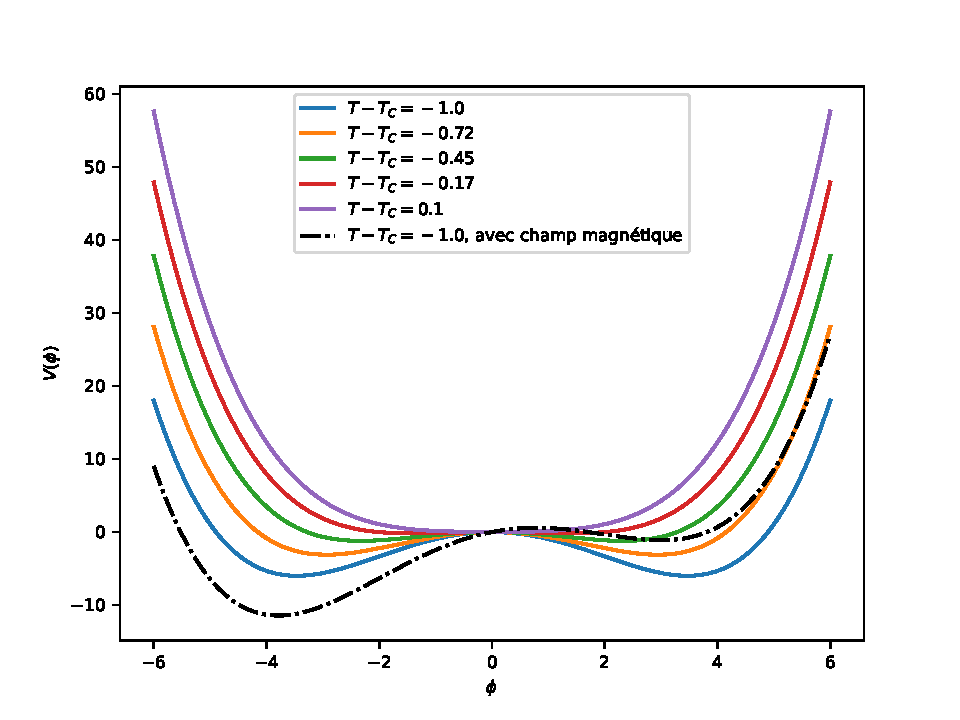
\includegraphics[width=0.6\linewidth]{intro/double-puit-en-fonction-temp.pdf}
    \caption{Potentiel en double-puits \ref{phi4} pour $\lambda=1$ en fonction de la différence entre la température et la température critique avec $m^2 = T-T_C$. Dans la phase ordonnée, les mimina stables sont à $\phi_C =\pm \sqrt{- \frac{6 m^2}{\lambda} } $, pour la phase désordonnée à $\phi_C = 0$. En noir, l'ajout d'un champ magnétique uniforme $h(\bx) = 1$ rend la phase positive métastable.}
    \label{double-puits-temperature}
\end{figure}


Now we return to dynamics. If we compare with systems with a discrete number of variables we
should have a Langevin equation of the form
\begin{equation}
    \frac{\partial \phi(\bx)}{\partial t}= -L \frac{\delta H}{\delta \phi(\bx)} + \eta(\bx,t).
\end{equation}
The white noise correlator should have the form
\begin{equation}
    < \eta(\bx,t)\eta(\bx',t)> =\delta(t-t')\Gamma(\bx,{\bf x'}),
\end{equation}
where here  $\Gamma(\bx,{\bf x'})$ is an operator (before it was a matrix) defined by its action on functions $f$ as
\begin{equation}
    \Gamma f(\bx) = \int d\bx' \Gamma(\bx,\bx')f(\bx'),
\end{equation}
and $L$ is also an operator with 
\begin{equation}
    L f(\bx) = \int d\bx' L(\bx,\bx')f(\bx'),
\end{equation}
Following the same arguments for systems with a finite number of degrees of freedom we thus have the relation (which is sometimes called the fluctuation dissipation theorem as it essentially is equivalent)
\begin{equation} 
    \Gamma(\bx,\bx') =2T L(\bx,\bx').\label{gnoise}
\end{equation}
The simplest form of dynamics is given by $L(\bx,\bx')=\alpha\delta(\bx-\bx')$ which gives the model A dynamics
\begin{equation}
    \frac{\partial \phi(\bx)}{\partial t}= -\alpha \frac{\delta H}{\delta \phi(\bx)} + \eta(\bx,t),    \label{MA}
\end{equation}
with the noise correlator
\begin{equation}
    < \eta(\bx,t)\eta(\bx',t)> =2T \alpha \delta(t-t')\delta(\bx-{\bf x'}).
\end{equation}
The average value of $\phi$ 
\begin{equation}
    \overline \phi(t) = \frac{1}{V}\int d\bx\  \phi(\bx,t),
\end{equation}
is clearly not generally conserved by this dynamics.

Model $B$ dynamics amounts to choosing
\begin{equation}
    L(\bx-\bx')= -D\nabla^2 \delta(\bx-{\bf x'}),
\end{equation}
here the fact that $L$ is a positive semi-definite operator can be seen by taking its Fourier transform. The evolution equation here is
\begin{equation}
    \frac{\partial \phi(\bx)}{\partial t}= D\nabla^2 \frac{\delta H}{\delta \phi(\bx)} + \eta(\bx,t),
    \label{MB}
\end{equation}
and where
\begin{equation}
    < \eta(\bx,t)\eta(\bx',t)> =-2TD   \delta(t-t')\nabla^2\delta(\bx-{\bf x'}).
\end{equation}
We notice that if we introduce the vectorial white noise with components $\eta_i(\bx,t)$ such that
\begin{equation}
    < \eta_i(\bx,t) \eta_i(\bx',t')> =\delta_{ij} \delta(\bx-{\bf x'})\delta(t-t),
\end{equation}
where $\delta_{ij}=1$ for $i=j$ and is zero otherwise,  we can write
\begin{equation}
    \eta(\bx,t)= \nabla\cdot {\boldsymbol \eta}(\bx,t),
\end{equation}
as one can verify the two noises have the same correlation function. In this way Eq. (\ref{MB}) becomes 
\begin{equation}
    \frac{\partial \phi(\bx)}{\partial t}= \nabla\cdot[ D\nabla \frac{\delta H}{\delta \phi(\bx)} +         {\boldsymbol\eta}(\bx,t)].
\end{equation}
From this it is easy to see that the order parameter is conserved - thus model  B describes conserved phase ordering dynamics.


%%%%%%%%%%%%%%%%%%%%%
    \subsection{Surface tension}
%%%%%%%%%%%%%%%%%%%%%

If there is non constraint on the system if can simply chose $\phi(\bx) =\phi_c$ or $\phi(\bx) =-\phi_c$ everywhere which corresponds to a  free energy $F=H[\phi_c]=0$. However in a system with a conserved order parameter
\begin{equation}
    \int d\bx \  \phi(\bx)=0, 
\end{equation}
then the solutions $\phi=\pm \phi_c$ cannot hold. In this case the system will separate into a two phases where $\phi(\bx)= \pm \phi_c$. We therefore choose an interface at $z=0$ where 
and take $\phi(\bx) = \phi_K(z)$ ($K$ standing for kink as it is known as the kink solution in the literature) where $\lim_{z\to\-\infty}=-\phi_c$ and  $\lim_{z\to\infty}=-\phi_c$. 
We therefore find from Eq. (\ref{cm}) that
\begin{equation}
    -\kappa \frac{d^2 }{dz^2}\phi_K(z)  + V'(\phi_K) = 0 \label{kk0}
\end{equation}
This equation can be solved for the potential in \eqref{p4} ({\em you should do it and fill in the details}) but even without knowing the explicit solution we can write
\begin{equation}
    H[\phi_K]=  A\int dz \ \frac{\kappa}{2}\left(\frac{d\phi_K(z)}{dz}\right)^2 + V(\phi_K(z)),\label{kk1}
\end{equation}
where $A$ is the surface area of the system in the plane perpendicular to the direction $z$. 
However if we multiply Eq. \eqref{kk0} by $d\phi/dz$ and integrate we find
\begin{equation}
    -\frac{\kappa}{2} (\frac{d\phi_K}{dz})^2 + V(\phi_K) = C,
\end{equation}
where $C$ is a constant. However as $\phi_K(z)\to \pm \phi_c$ as $z\to \pm \infty$ and $V(\pm\phi_c) =0$ we find that $C=0$. Using this we obtain 
\begin{equation}
    H[\phi_K]=  A\int dz\  {\kappa}\left(\frac{d\phi_K(z)}{dz}\right)^2 .
\end{equation}
If the interface has a free energy per unit area of $\sigma$ then we have the Cahn-Hillard estimate of the surface tension 
\begin{equation}
    \sigma=  \int dz\  {\kappa}\left(\frac{d\phi_K(z)}{dz}\right)^2 .\label{CHST}
\end{equation}

Dans le cas du modèle $\phi^4$ définie à l'équation \ref{phi4}, l'équation \ref{kink} devient
\begin{align}
    \kappa \phi_K''(z) = m^2 \phi_K(z) \left( 1 + \phi_C \phi_K(z) ^2 \right)
       \label{eq-interface-glauber}
\end{align}
Dans le modèle, le comportement est seulement déterminé par le ratio entre $m^2$ et $\lambda$. Posons donc sans perte de généralité $\phi_C = 1$. La solution est  
\begin{align}
    \phi_K(z) = \phi_C \tanh \left( \frac{z}{\xi} \right)
       \label{profil-interface-glauber}    
\end{align}
où $\xi = \sqrt{\frac{-2 \kappa}{m^2}}$. Cette longueur de corrélation diverge lorsque $T \to T_C$. On remarque que pluys la longueur de corrélation augmente, plus la dérivée de l'interface est faible, menant à une diminution de la tension superficielle \ref{tension-superficielle}. Aussi, l'étude expérimentale des systèmes quasi-critiques est une porte d'accès pour l'étude des systèmes à ultra basse tension superficielle \cite{hennequin_drop_2006}. De tels systèmes sont extrêmement sensibles aux instabilités hydrodynamiques causées par l'agitation thermique, présentant de nombreuses applications en microfluiidque par exemple \cite{atencia_controlled_2005}. 


%%%%%%%%%%%%%%%%%%%%%%
\section{Models for equilibrium interfaces}
%%%%%%%%%%%%%%%%%%%%%%

Here we discuss effective models of interfaces. The simplest model is to assume that the 
interface is parameterised by a height profile $h(\br)$, however one also has to assume that 
$h(\br)$ is a single valued function of $\br$. Given this one can write
\begin{equation}
    H[h] = \sigma A[h]
\end{equation}
where $A_h$ is the area of the interface. However the interface area is given by
\begin{equation}
    A[h] = \int_A d\br\sqrt{1+[\nabla h]^2},
\end{equation}
where the integral is over the plane perpendicular to the $z$ axis which is taken to be of area $A$. When the fluctuations of the interface are small, we can expand the above to quadratic order in $h$ to obtain
\begin{equation}
    H[h]= A\sigma +\frac{\sigma}{2} \int_A d\br \ [\nabla h]^2.
\end{equation}
The first term is independent of the height so we can write the effective Hamiltonian for the surface as
\begin{equation}
    H_{eff} [h]= \frac{\sigma}{2} \int_A d\br\  [\nabla h]^2.
    \label{heff}
\end{equation}

The basic model describing the height of an interface at $z=h(\bx)$ above a plane with coordinates $\bx$ has the Hamiltonian 
\begin{equation}
    H[h] = \int d\bx\frac{\sigma}{2} [\nabla h(\bx)]^2 + V(h(\bx)).
\end{equation}
The first term corresponds to the surface energy for a surface of size $A_s$ 
\begin{equation}
    H_s[h] = \sigma A_s =\sigma\int d\bx \sqrt{1+[\nabla h(\bx)]^2}\approx \sigma A + \frac{\sigma}{2}\int d\bx [\nabla h(\bx)]^2 .
\end{equation}
Here $A$ is the area of the projected plane below the surface which is taken to be constant and thus does not change the statistical mechanics of the system. In principle surfaces can also have bending energies, while surface energies correspond to stretching the surface to increase its size, bending energies correspond to curving the surface. The standard bending energy for small surface energies is given by
\begin{equation}
    H_b[h] = \int d\bx \frac{\kappa_b}{2}[\nabla^2 h(\bx)]^2,
\end{equation} 
where $\kappa_b$ is called the bending rigidity.

The term $V(h)$ is taken to represent the potential energy of the surface. For instance if the surface interacts via an infinite hard core potential with a solid surface at $z=0$, this can be modelled by the potential $V(z) =0$ for $z>0$ and $V(z)=\infty$ for $z\leq 0$. Another example is where the surface describes the surface of a liquid such as water, again with a solid surface at $z=0$, in the presence of gravity the potential energy of the water column above the area 
element $d\bx$ is given by
\begin{equation}
    \delta V = \int_0^{h(\bx)} dz\ \rho g z = \frac{1}{2}\rho g h^2(\bx),
\end{equation}
where $\rho$ is the (mass) density of the liquid. This then gives
\begin{equation}
    H[h] = \int d\bx \frac{\sigma}{2}[\nabla h(\bx)]^2 + \frac{1}{2}\rho g h^2(\bx).
\end{equation}
We see that the correlation length of the interface is given by
\begin{equation}
    \xi = \left(\frac{\sigma}{\rho g}\right)^{\frac{1}{2}}.
\end{equation}
In the more general context if $V(h)$ has a minimum at some point $h_m$ we can write $h= h_f(\bx)+ h_m$, where  $h_f(\bx)$ represents the height fluctuations about the mechanically stable flat interface $h(\bx)=h_m$. Now expand assuming that $h_f(\bx)$ is
small we find the effective Hamiltonian for the fluctuations
\begin{equation}
    H_{eff}[h_f] = \int d\bx \frac{\sigma}{2}[\nabla h_f(\bx)]^2 + \frac{1}{2}V''(h_m) h_f^2(\bx),
\end{equation}
where we have dropped the constant term $AV(h_m)$. The above field theory is Gaussian and 
so, when the approximations made to derive it are valid, all of the statistical properties of the height fluctuations can be deduced. However for general potentials $V(h)$ the model cannot be solved exactly in two dimensions but can in principle be solved in one dimension as we will see below.


%%%%%%%%%%%%%%%%%%%%%%
    \section{Effective dynamics of interface heights}\label{heightd}
%%%%%%%%%%%%%%%%%%%%%%
We will now try and derive an approximation for the dynamics of the  height of the interface from the original phase ordering kinetics. Here we use the method of Bray and Cavagnha - put in the reference, which was used to study the dynamics of sheared interfaces, in the absence of shear to determine the dynamical properties of interfaces in phase separated systems for both model A and model B dynamics.

We imagine that the system is phase separated in the direction  $z$, on average the interface is taken to be at $z=0$, and we write
\begin{equation}
    \phi(z,\br,t) = f(z-h(\br,t))\label{hans}
\end{equation}
where $f(z)=\phi_K(z)$ is the kink solution from mean field theory.

%%%%%%%%%%%%%%%%%%
    \subsection{Model A dynamics}
%%%%%%%%%%%%%%%%%%

For model A dynamics, we substitute Eq. \eqref{hans} into Eq. \eqref{MA} and make use of the following results
\begin{eqnarray}
\frac{\partial f(z-h(\br,t))}{\partial t}&=& -f'(z-h(\br,t))\frac{\partial h(\br,t)}{\partial t}\\
\nabla f(z-h(\br,t))&=& [{\bf e}_z-\nabla h(\br,t)]f'(z-h(\br,t))  \\
\nabla^2 f(z-h(\br,t))&=& f''(z-h(\br,t))- \nabla^2 h(\br,t)f'(z-h(\br,t))+ [\nabla h(\br,t)]^2 
f''(z-h(\br,t))
\end{eqnarray}
and thus find
\begin{eqnarray}
&&-f'(z-h(\br,t))\frac{\partial h(\br,t)}{\partial t}= \alpha\kappa\times\\ &&\left[f''(z-h(\br,t))- \nabla^2 h(\br,t)f'(z-h(\br,t))+ [\nabla h(\br,t)]^2 
f''(z-h(\br,t))\right] - \alpha V'(f'(z-h(\br,t))) + \eta(\br,z,t).
\end{eqnarray}
We now multiply both sides of this equation by $f'(z-h(\br,t))$ and defining $\zeta=z-h(\br,t)$ we integrate  $\zeta$ over $[-\infty,\infty]$ and use the following identities
\begin{eqnarray}
\int_{-\infty}^\infty d\zeta f'(\zeta)f''(\zeta) &=& [\frac{1}{2}f'^2(\zeta)]_{-\infty}^\infty =0\\
\int_{-\infty}^\infty d\zeta f'(\zeta) V'(f) &=& \int_{-\infty}^\infty d\zeta\frac{d V(f)}{d\zeta}= [V(f(\zeta))]_{-\infty}^\infty=0,
\end{eqnarray} 
note that the first relation above holds as $f(\zeta)=\pm \phi_c$ as $\zeta\to\pm \infty$ and the second as
$V(\phi_c)=V(-\phi_c)=0$.
The terms that are left then give
\begin{equation}
    -\int_{-\infty}^\infty f'^2(\zeta)d\zeta\ \frac{\partial h(\br,t)}{\partial t}
    = -\alpha\int_{-\infty}^\infty f'^2(\zeta)d\zeta \ \kappa \nabla^2 h(\br,t) + \int_{-\infty}^\infty d\zeta \eta(\br,\zeta+ h(\br,t))f'(\zeta)
\end{equation}
Now using the Cahn-Hillard estimate of the surface tension Eq. \eqref{CHST} this becomes
\begin{equation}
    \frac{\sigma}{\kappa} \frac{\partial h(\br,t)}{\partial t}
    = \alpha\sigma \nabla^2 h(\br,t) +\xi(\br,t),
\end{equation}
where the noise term is given by
\begin{equation}
    \xi(\br,t)= \int_{-\infty}^\infty d\zeta \eta(\br,\zeta+ h(\br,t))f'(\zeta)
\end{equation}
The noise term has zero mean and correlation function
\begin{eqnarray}
< \xi(\br,t)\xi(\br',t')> &=&2\alpha T\delta(t-t')\delta(\br-\br')\int_{-\infty}^\infty d\zeta d\zeta' \delta(\zeta-\zeta')f'(\zeta)f'(\zeta')\\
&=& 2\alpha T\delta(t-t')\delta(\br-\br')\int_{-\infty}^\infty d\zeta f'^2(\zeta)= \frac{2\alpha T\sigma}{\kappa}\delta(t-t')\delta(\br-\br').
\end{eqnarray}
This now gives
\begin{equation}
    \frac{\partial h(\br,t)}{\partial t}= \kappa\alpha \nabla^2 h(\br,t) + \eta(\br,t)
\end{equation}
where 
\begin{equation}
    < \eta(\br,t)\eta(\br',t')> = \frac{2\alpha T\kappa}{\sigma}\delta(t-t')\delta(\br-\br').
\end{equation}
Now defining $\alpha' = \frac{\kappa\alpha}{\sigma}$ we can write
\begin{equation}
    \frac{\partial h(\br,t)}{\partial t}= \alpha' \sigma\nabla^2 h(\br,t) + \eta(\br,t).
\end{equation}
This has the form of model $A$ dynamics (as in Eq. \eqref{MA})  for the height profile with Hamiltonian
$H_{eff}$ as given in \eqref{heff}, that is to say we can write
\begin{equation}
    \frac{\partial h(\br,t)}{\partial t}= -\alpha' \frac{\delta H_{eff}[h]}{\delta h(\br)} + \eta(\br,t),
    \label{ew}
\end{equation}
and where 
\begin{equation}
    < \eta(\br,t)\eta(\br',t')>= 2T\alpha'\delta(t-t').
\end{equation}
This dynamical calculation is thus consistent with the idea of describing the surface in terms of a height variable with an energy given by the surface tension. The equation \eqref{ew} is known as the Edwards-Wilkinson equation. We can use this equation to determine how the domains of a coarsening systems grow at low temperatures. To do this we ignore the noise term and assume that at $t=0$ the correlations of the height are short range so
\begin{equation}
    C(\br-\br',0)= < h(\br,0)h(\br',0)> =C_0 \delta(\br-\br').
\end{equation}
In Fourier space the noiseless Edwards-Wilkinson equation becomes
\begin{equation}
    \frac{\partial\tilde h(\bk,t)}{\partial t} = -\alpha'\sigma \tilde h(\bk,t) ,
\end{equation}
and so we find
\begin{equation}
    \tilde h(\bk,t) = h(\bk,0)\exp(-\alpha'\sigma\bk^2 t).
\end{equation}
We thus find 
\begin{equation}
    < \tilde h(\bk,t)\tilde h(\bk',t')> = < h(\bk,0)h(\bk',0)> \exp(-    \alpha'\sigma[k^2+k'^2] t).
\end{equation}
Now recall that if 
\begin{equation}
    <  h(\br,t) h(\br',t')> =C(\br-\br',t)
\end{equation}
then
\begin{equation}
    < \tilde h(\bk,t)\tilde h(\bk',t')>= (2\pi)^d \delta(\bk+\bk') \tilde C(\bk,t),
\end{equation}
where 
\begin{equation}
    \tilde C(\bk,t)= \int d\br \exp(-i\bk\cdot \br)C(\br,t),
\end{equation}
is the Fourier transform of the correlation function which is a function of a single position due to invariance by translation in space, and $d$ is the dimension of space (so here $d=2$ for a surface in 3d space and $d=1$ for a surface in a 2d space). Putting all this together gives
\begin{equation}
    \tilde C(\bk,t)= C_0 \exp(-2\alpha'\sigma k^2 t).
\end{equation}
Inverting the Fourier transform gives
\begin{equation}
    C(\br,t)= \frac{C_0}{(8\pi \alpha'\sigma t)^{\frac{d}{2}}} \exp(-\frac{\br^2}{16\pi \alpha'\sigma t}).
\end{equation}
From this we see that if $C(\br,t)\sim g(\frac{\br}{\ell(t)})r(t)$ then the length scale $\ell(t)\sim t^{\frac{1}{2}}$, this agrees with is found in the Ising model under Glauber dynamics, where the growth exponent is also given by $z=\frac{1}{2}$.

%%%%%%%%%%%%%%%
    \subsection{Model B dynamics}
%%%%%%%%%%%%%%

For model B dynamics, we take the same ansatz as in Eq. \eqref{hans} but we rewrite the model B dynamics as
\begin{equation}
    -\nabla^{-2} \frac{\partial\phi(\bx,t)}{\partial t} = -D \frac{\delta H}{\delta \phi(\bx)}+ 
    \theta(\bx,t),
\end{equation}
here $-\nabla^{-2}$ represents the Green's function $G$ which obeys 
\begin{equation}
    \nabla^2 G(\bx-{\bf x'}) = -\delta(\bx-\bx'),
\end{equation}
and 
\begin{equation}
    \theta(\bx,t)=-\nabla^{-2}\eta(\bx,t)= \int d\bx'G(\bx-{\bf x'})\eta(\bx,t)
\end{equation}
The correlation function of $\theta(\bx,t)$ is given by
\begin{eqnarray}
< \theta(\bx,t)\theta({\bf y},t')> &=&-2DT\delta(t-t') \int d\bx'G(\bx-{\bf x'})d{\bf y}'G({\bf y}-{\bf y'})\nabla^2\delta(\bx'-{\bf y}') \\
&=& -2DT\delta(t-t') \int d\bx'G(\bx-{\bf x'})d{\bf y}'\nabla^2G({\bf y}-{\bf y'})\delta(\bx'-{\bf y}') \\
&=& 2DT\delta(t-t') G(\bx-{\bf y}).
\end{eqnarray}
where we have integrated by parts in the second line and used 
\begin{equation}
    -\nabla^2G({\bf y}-{\bf y'})= \delta({\bf y}-{\bf y}'),
\end{equation}
in the third.

Now mutliplying by $f'(z-h(\br,t))$ and integrating $z$ over $[-\infty,\infty]$, we find
\begin{eqnarray}
&&-\int dz f'(z-h(\br,t))\int dz'd\br'\  G(z-z',\br-\br') f'(z'-h(\br',t))\frac{\partial h(\br',t)}{\partial t} = \\
&&-D\sigma \nabla^2 h(\br,t) + \chi(\br,t),
\end{eqnarray}
with the noise
\begin{equation}
    \chi(\br,t)= \int dz f'(z-h(\br,t)) \theta(\br,z,t).
\end{equation}
As we assume that the height fluctuations are small we keep only the lowest order terms in $h$ in the deterministic terms and the noise, we will see later that this is compatible thermodynamically. We thus have
\begin{eqnarray}
&&-\int dz \ f'(z)\int dz'd\br'\  G(z-z',\br-\br') f'(z')\frac{\partial h(\br',t)}{\partial t} = \\
&&-D\sigma \nabla^2 h(\br,t) + \chi(\br,t),
\end{eqnarray}
and now  the noise is given by
\begin{equation}
    \chi(\br,t)= \int dz\  f'(z) \theta(\br,z',t).
\end{equation}
This equation which is linear in $h$ can now be Fourier transformed in the plane $\br$ and in terms of the Fourier transform of $h$ we find
\begin{equation}
    -\int dz \ f'(z)\int dz'd\br'\ \tilde G(z-z',\bk) f'(z')\frac{\partial\tilde h(\bk,t)}{\partial t} = Dk^2\sigma \tilde h(\bk,t) + \tilde \chi(\bk,t).
    \label{bstep}
\end{equation}
The Fourier transform of $G$ in the $\br$ plane obeys
\begin{equation}
    \frac{d^2 \tilde G(z-z',\bk )}{dz^2}-k^2 \tilde G(z-z',\bk )=-\delta(z-z')
\end{equation}
and the solution to this equation (with the boundary condition that $\tilde G(z-z',\bk )\to 0$ as $|z-z'|\to\infty$)  is
\begin{equation}
    \tilde G(z-z',\bk) = \frac{\exp(-k|z-z'|)}{2k},
\end{equation}
and note that $k=|\bk|$. 
Next we make the sharp interface approximation where we write
\begin{equation}
    f(z) = 2\phi_c \delta(z),
    \label{sharp}
\end{equation}
that is to say we have replaced the smooth kink solution with a step like solution
$f(z) = \phi_c\  {\rm sgn}(z)$. This then gives
\begin{equation}
    -4\phi_c^2 \tilde G(0,k) \frac{\partial h(\bk,t)}{\partial t} = Dk^2\sigma  \tilde h(\bk,t) + \tilde \chi(\bk,t),
\end{equation}
which we rewrite as
\begin{equation}
    \frac{\partial \tilde h(\bk,t)}{\partial t} = -\frac{Dk^3\sigma}{2\phi_c^2} \tilde h(\bk,t) + \tilde \xi(\bk,t),
\end{equation}
with 
\begin{equation}
    \tilde \xi(\bk,t)= - \frac{k}{2\phi_c^2}\tilde \chi(\bk,t),
\end{equation}
where 
\begin{equation}
    \tilde \chi(\bk,t)= \int dz\  f'(z) \tilde\theta(\bk,z,t),
\end{equation}
The correlation function of $\tilde \theta(\bk,t)$ is 
\begin{equation}
    < \theta(\bk,t)\theta(\bk',t')> = 2DT(2\pi)^d \delta(t-t') \delta(\bk+{\bf k'}) \tilde G(z-z',k)
\end{equation}
and from this we find 
\begin{equation}
    < \chi(\bk,t)\chi(\bk',t')>  = 2DT(2\pi)^d \delta(t-t') \delta(\bk+{\bf k'}) \int dz dz' f(z) f(z') \tilde G(z-z',k),
    \label{bstep2}
\end{equation}
now using the sharp interface approximation Eq. (\ref{sharp}) we obtain
\begin{equation}
    < \chi(\bk,t)\chi(\bk',t')>  = 2DT(2\pi)^d \delta(t-t') \delta(\bk+{\bf k'}) \frac{2\phi_c^2}{k},
\end{equation}
and consequently
\begin{equation}
    < \xi(\bk,t)\xi(\bk',t')> = 2DT(2\pi)^d \delta(t-t') \delta(\bk+{\bf k'}) \frac{k}{  2\phi_c^2}.
\end{equation}
Finally in we find the interface dynamics for model B in Fourier space is
\begin{equation}
    \frac{\partial h(\bk,t)}{\partial t} = -\frac{Dk^3\sigma}{2\phi_c^2} \tilde h(\bk,t) + \tilde \xi(\bk,t),
    \label{modBFT}
\end{equation}
In real space this has the form
\begin{equation}
    \frac{\partial h(\br)}{\partial t}= -L \frac{\delta H_{eff}}{\delta h (\br)} + \xi(\br,t).
\end{equation}
where the operator $L$ is defined via its Fourier transform
\begin{equation}
    \tilde L(\bk) = \frac{Dk}{2\phi_c^2}.
\end{equation}
Now if we look at Eq. \eqref{modBFT} we see that solving the equation without noise will give a function of $k^3t$, which in real space corresponds to $x^3/t$. From this we see that the coarsening length scale grows as $\ell(t) \sim t^{\frac{1}{3}}$ and consequently the coarsening exponent is $z=\frac{1}{3}$.  Coarsening for conserved model B or diffusive dynamics is slower than that of model A. One of the reasons for this slowing down with respect to nonconserved dynamics is that material must be physically transported by diffusion (by exchanging spins in the language of lattice spin models), where as for  model A dynamics the composition can change at any given point by {\em spin flipping}. As a cautionary note, if we had taken the
Hamiltonian in Eq. \eqref{heff} and applied model B conserved dynamics, as in Eq. \eqref{MB},  for the height field we would not have obtained this equation. 

We can actually do better than the above sharp interface approximation as Eq. \eqref{bstep} can be written as
\begin{equation}
    Q(k)\frac{\partial\tilde h(\bk,t)}{\partial t} =  -Dk^2\sigma \tilde h(\bk,t) - \tilde \chi(\bk,t).
    \label{bstep2}
\end{equation}
where 
\begin{equation}
    Q(k)= \int dzdz' \ f'(z)\ \tilde G(z-z',\bk) f'(z').
\end{equation}
Notice that from Eq. \eqref{bstep2} that
\begin{equation}
    < \chi(\bk,t)\chi(\bk',t')>  = 2DT(2\pi)^d \delta(t-t') \delta(\bk+{\bf k'}) Q(k)\end{equation}
and so 
\begin{equation}
    \frac{\partial\tilde h(\bk,t)}{\partial t}= -\tilde L(k) \tilde \mu(\bk) + \eta(\bk),
\end{equation}
where $\mu(\bx)=\delta H_{eff}/\delta h(\bx) $ and $\tilde L(k) = D/Q(k)$ and 
\begin{equation}
    < \eta(\bk,t)\eta(\bk',t')>  = 2T(2\pi)^d \delta(t-t') \delta(\bk+{\bf k'}) \tilde L(k).
\end{equation}

%%%%%%%%%%%%%%%%%%%%%%
    \section{Systems driven by imposed hydrodynamic flows}
%%%%%%%%%%%%%%%%%%%%%%
{\bf Here you need to discuss the experiments get some nice photos etc}

Here we consider what happens when a system is driven out of equilibrium, by driven we mean that energy is injected into the system by a laser for instance as discussed in the introduction or by inducing a hydrodynamics flow, for instance a shear flow induced in a Couette cell. In principle we should analyse this system with model H dynamics which couples diffusive model B dynamics to hydrodynamics in the low Reynolds number Stokes flow regime. In this dynamics the order parameter field will itself induce a hydrodynamics flow which will modify
the imposed one. However this full situation is very difficult to analyse and to a first approximation we can assume that the back reaction of the order parameter field on the hydrodynamic flow is small with respect to the imposed hydrodynamic flow and so we can simply write
\begin{equation}
    \frac{\partial \phi (\bx,t)}{\partial t} + \nabla\cdot({\bf  v}(\bx)\phi(\bx,t)) =- L\frac{\delta H}{\delta \phi(\bx)} + \eta(\bx,t),
    \label{drive}
\end{equation}
where $L$ is given by the underlying model A or B dynamical operatorand the noise has the correlation function as given by Eq. \eqref{gnoise}, and ${\bf v}(\bx)$ is the imposed (time independent) hydrodynamic flow or can equally well be an external drive imposed on the colloidal particles, due to the gravitational or electric field for example. 

The simplest case one can consider is where the driving field ${\bf v}(\bx) ={\bf v}_0$ is uniform . Unfortunately this simple driving does not lead to a new steady state. Basically all of the colloidal particles acquire an an average velocity ${\bf v}$ and so move along at the same speed relative to each other. Mathematically this can be seen by making the Galilean transformation
\begin{equation}
    \phi (\bx,t)= \phi(\bx-{\bf v}_0t,t) = \phi({\bf y},t).
\end{equation}
this transform eliminates the driving from the evolution equation \eqref{drive} and so we find an equilibrium system. 

The most studies example is where the driving is a shear flow, this corresponds to the experiments of Derks et al and the numerical simulations of Smith et al and the analytical work
of Bray and Cavagnah. In Bray and Cavagna, the effective dynamics of the surface term 
in the presence of a shear flow, parallel to the interface,
\begin{equation}
    {\bf v}(\bx) = \gamma z {\bf e}_x
\end{equation}
was studied using the method explained in section (\ref{heightd}). The addition of a shear flow leads to the appearance of a nonlinear term in $h$ and the interface statistics thus become non-Gaussian.

\begin{figure}
	\begin{minipage}[t]{0.5\linewidth}
		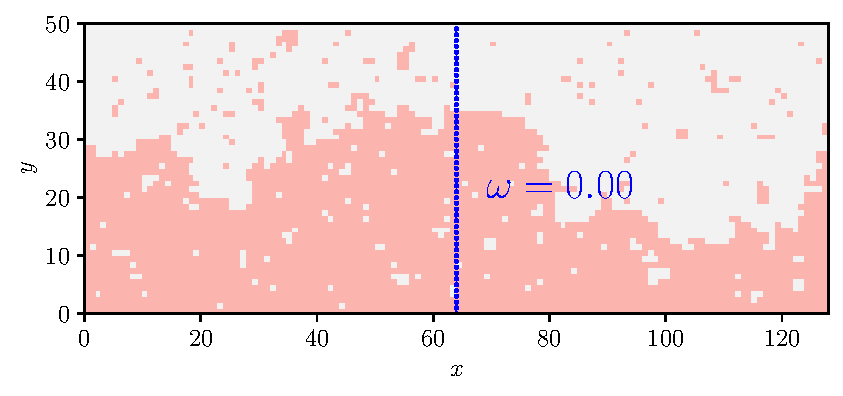
\includegraphics[width=\linewidth]{intro/cis-ising-f-000.pdf}
	\end{minipage}%
	\begin{minipage}[t]{0.5\linewidth}
		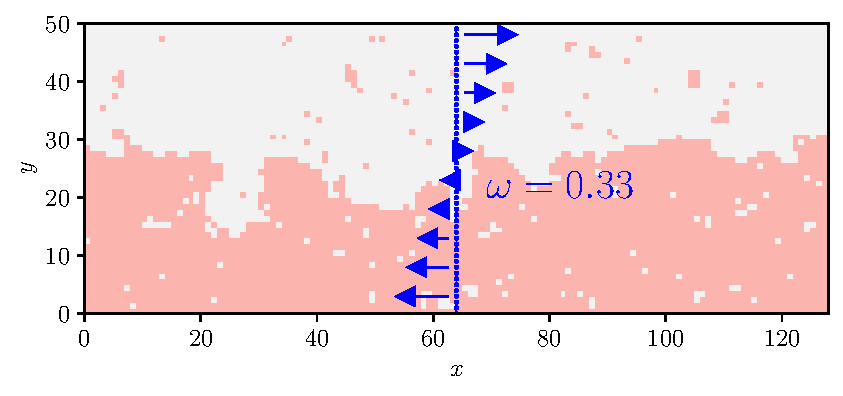
\includegraphics[width=\linewidth]{intro/cis-ising-f-033.pdf}
	\end{minipage}
	\centering
	\begin{minipage}[t]{0.5\linewidth}
		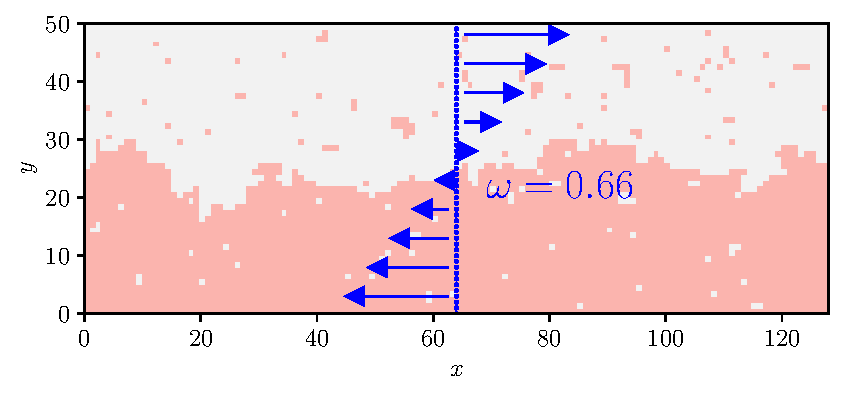
\includegraphics[width=\linewidth]{intro/cis-ising-f-066.pdf}
	\end{minipage}
	\caption{Photos d'un système d'Ising en fonction du cisaillement  \ref{eq-cisaillement} via des simulations de Monte Carlo avec un algorithme de Kawasaki. Ledit algorithme sera expliqué plus en détail au chapitre \ref{chap-sim}.}
    \label{snap-ising-shear}	
\end{figure}  

%%%%%%%%%%%%%%%%%%%
    \section{Lattice models}
%%%%%%%%%%%%%%%%%%%
Comme indiqué dans l'équation \ref{renormalisation},  le champ $\phi(\bx,t)$ est un champ moyenné sur le temps et l'espace à cause de la précision de nos appareils de mesure. Si par exemple le champ $\phi$ représente une densité de particules, alors au niveau le plus fondamental, le champ est charactérisé par
\begin{align}
    \phi(\bx,t) = \frac{1}{V} \sum_i \delta(\bx-\bx_i(t) 
\end{align}
où $V$ est le volume d'inégration défini par la précision de notre mesure et $\bx_i(t)$ est la position de la particule $i$ à l'instant $t$.  Ainsi à l'échelle des constituants du système, le champ est discontinu. Cette discontnuité inhérente du système microscopique nous mène naturrellement sur des modèles de particules sur réseau. 
Dans les modèles sur réseau, nous fixons un ensemble de positions $\{\bx_i\}$ que les particules peuvent occuper, puis nous regardons l'évolution temporelle d'un tel système en fonctoins des interactions désirées entre les sites.

Nous nous intéressons ici aux modèles sur réseaux cubiques, de taille $L' \times L' \times L$, dont le modèle d'Ising est le plus connu. Nous développons les principaux résultats obtenus dans les modèles d'Ising pour la force de Casimir critique et l'importance des forces de cisaillement sur les propriétés des interfaces.
Puis nous expliquerons un modèle à $(d-1)$ dimension du modèle d'Ising à basse température, le \textbf{modèle Solid-On-Solid} (SOS), avec les techniques propres au système 1D de la matrice de transfert ainsi que les propriétés analytiques de l'interface déjà connues.
 
La discrétisation du champ $\phi(\bx,t)$ afin de faire des simulations numériques mène naturellement vers le modèle sur réseau par excellence, le modèle d'Ising. À partir de deux dimensions, ce modèle de particules à interaction avec les plus proches voisins, possède une transition de second ordre depuis une phase ordonnée vers une phase désordonnée. Si lon suppose l'énergie d'interactiosn entre toutes les particules plus proches voisins égale à $J$, la température critique est $\beta_{C,2D} =  \frac{\ln(1+\sqrt{2})}{2} J \simeq 0.44 J$ en deux dimensions \cite{onsager_crystal_1944}. et $\beta_{C,3D} \simeq 0.22 J$ en trois dimensions \cite{talapov_magnetization_1996} (via des simulations de Monte Carlo).

%%%%%%%%%%%%%%%%%%%%%%%%%%%%%%%%%%%%%%%%%%%%%
    \subsection{Le modèle d'Ising}
%%%%%%%%%%%%%%%%%%%%%%%%%%%%%%%%%%%%%%%%%%%%%  
\begin{figure}
	\begin{minipage}[t]{0.5\linewidth}
		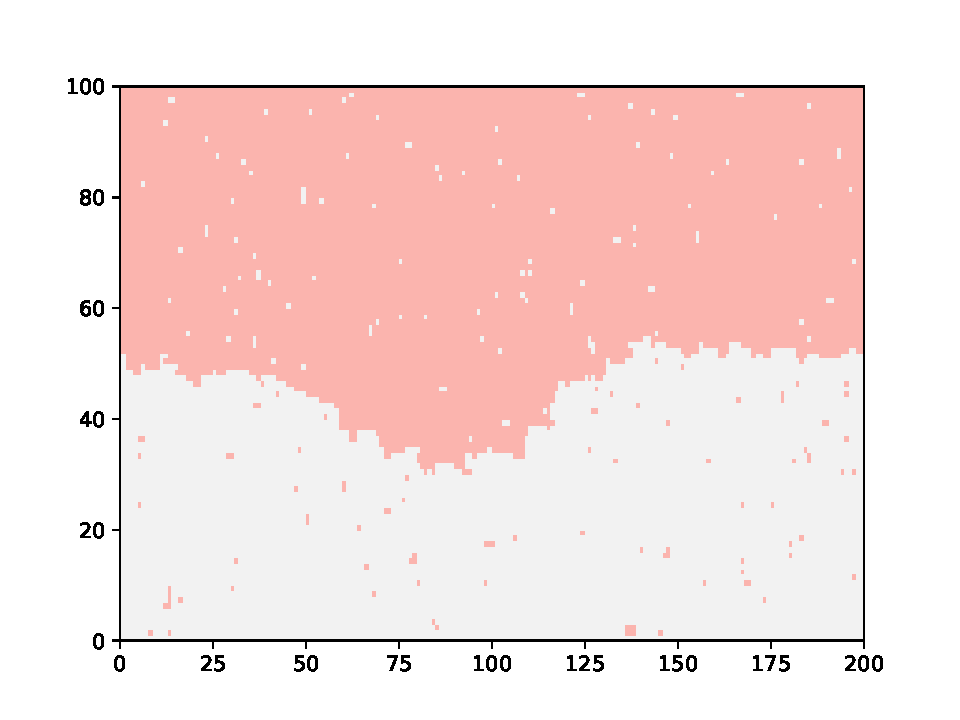
\includegraphics[width=\linewidth]{int-dyn/inte07.pdf}
	\end{minipage}%
	\begin{minipage}[t]{0.5\linewidth}
		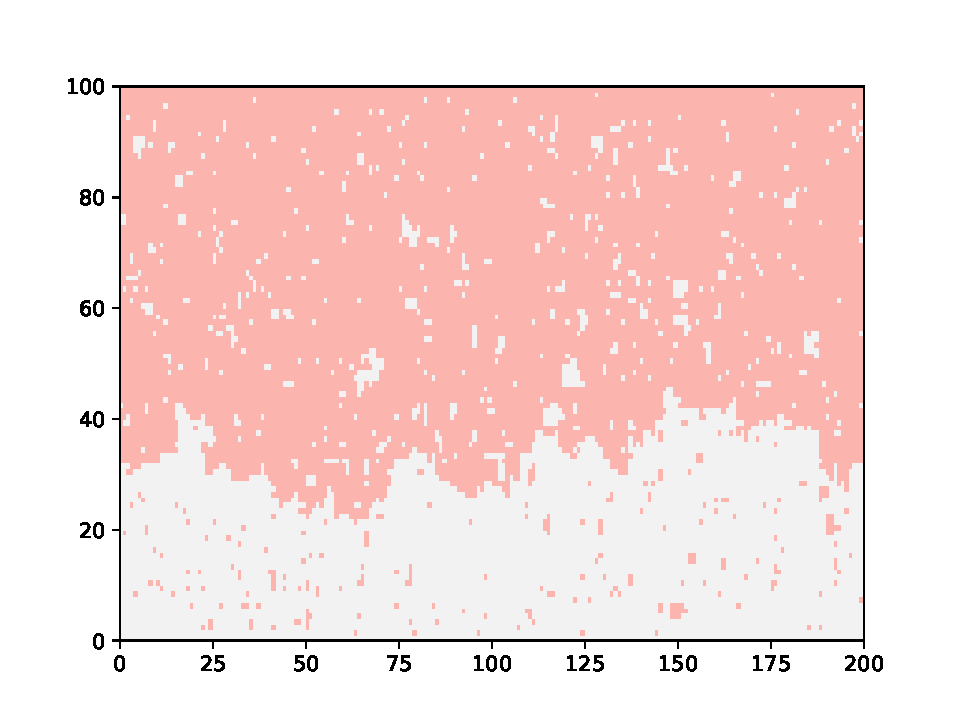
\includegraphics[width=\linewidth]{int-dyn/inte09.pdf}
	\end{minipage}
	\caption{Photo d'un modèle d'Ising pour deux températures différentes($T=0.7 T_C$ et $T=0.95 T_C$ ) avec des conditions périodiques aux bords en X et fixés en Y qui forcent la présence d'une interface entre les phases $+$ (rose) et $-$ (blanc) du système. Plus la température est élevée et plus l'interface fluctue, jusqu'à cesser d'exister pour $T \greater T_C$. }
	\label{amas-fixe}
\end{figure}  

Nous rappelons l'Hamiltonien \ref{hamil-mean-field} du champ moyen 
\begin{align}
    H[\phi] = \int d \bx  \frac{\kappa}{2}[{\boldsymbol \nabla} \phi]^2 + V(\phi)
\end{align}
où $V(\phi)$ est un potentiel de possédant deux minima en $\phi_C = \pm1$. On considère maintenant que le champ sur les sites de notre réseau est égal à $\pm \phi_C = \pm 1$. On note ${\bf i}:=(x,y,z)$ le site du réseau correspondant aux coordonnées $(x,y,z)$. Sur un réseau carré discret de pas $a=1$, la discrétisation du premier terme au premier ordre se traduit par 
\begin{align}
    [{\boldsymbol \nabla} \phi({\bf i})]^2 &= \left( \frac{\partial \phi({\bf i})}{\partial x} \right)^2  + \left( \frac{\partial \phi({\bf i})}{\partial y} \right)^2 + \left( \frac{\partial \phi({\bf i})}{\partial z} \right)^2\nn
    &= (\phi(x,y,z)-\phi(x+1,y,z))^2 + (\phi(x,y,z)-\phi(x,y+1,z))^2 + (\phi(x,y,z)-\phi(x,y,z+1))^2 \nn
    &= 2 (1-\phi(x,y,z)\phi(x+1,y,z) + 2 (1-\phi(x,y,z)\phi(x,y+1,z) +2 (1-\phi(x,y,z)\phi(x,y,z+1) 
    \label{discretisation-landau}
\end{align}
Notons $\sigma_i = \phi({\bf i}) = \pm 1$, et $J := \kappa$. On obtient alors l'Hamiltonien du modèle d'Ising
\begin{equation}
	H =  - \sum_{<i j >} J \sigma_i \sigma_j + \frac{V(\sigma_i)+V(\sigma_j)}{2}
	\label{hamil-ising}
\end{equation}
où $\sum_{< ij >}$ est une somme sur toutes les paires de premiers voisins. Le champ externe $V(i)$ a ici été symmétrisé et le terme constant de \ref{discretisation-landau} a été retiré.
Le modèle d'Ising\cite{niss_history_2005,niss_history_2009} est donc un modèle sur réseau à interactions courtes entre les particules. Puisque les constituants $\sigma_i$ du système sont tous égaux à $\pm!$, on appelle ce système un système de spin sur réseau. Dans le cas où la variable $\sigma_i$ est continue, on parle de modèle XY. Pour plus de généralité, il est également possible de varier l'interaction entre les plus proches voisins en posant $J = J_{ij}$. Si $ J_{ij} =0$, on parle d'interaction ferromagnétique favorisant à homogénéiser le système malgré l'agitation thermique. Si  $J_{ij} < 0$, on parle d'interaction antiferromagnétique favorise les systèmes où chaque spin possède un signe différent de celui de tous ses plus proches voisins. On prendra pour le reste de cette thèse $J=1$.

Ce modèle décrit précisément les transitions de phases dans les matériaux magnétiques uniaxiaux \cite{de_jongh_experiments_1974,wp_wold_ising_2000,ikeda_neutron_nodate}. Il est par ailleurs le modèle le plus simple à l'intérieur de sa classe d'universalité, qui contient également les transitions liquide/gaz ainsi que l'émulsion de liquides binaires. Ce modèle ne possède pas de transitions de phase en une dimension. La solution en deux dimensions a été trouvée par \cite{onsager_crystal_1944}, prouvant l'existant d'une transition de phase à 
\begin{align}
     T_{2D,C} = \frac{2J}{k_B \ln(1 + \sqrt{2})} \simeq 2.27 \frac{J}{k_B}
\end{align}
Puisque ce modèle découle de la discrétisation du champ moyen, ces approches donnent beaucoup d'informations sur la transition de phase et ses propriétés au point critique en 4 dimensions et au-delà, avec $d=4$ étant la dimension critique supérieure. Cependant le modèle n'a pas encore été résolu pour $d=3$, bien que de nombreuses simulations numériques \cite{preis_gpu_2009} ont permis de trouver que la transition critique était à
\begin{align}
    T_{3D,C} \simeq 4.51 \frac{J}{k_B}
\end{align}

En faisant la transformation\cite{goldenfeld_lectures_2018} 
\begin{align}
    n_i =  \frac{\sigma_i +1}{2}
\end{align}
afin que $n_i(\sigma_i = 1) = 1$ et $n_i(\sigma_i = -1) = 0$, on obtient l'Hamiltonien
\begin{equation}
	H =  - \sum_{< i j >}  J_{ij} \left( 4 n_i n_j -2 ( n_i+n_j) + 1 \right)+ \sum_{< i j >}  J_{ij} \frac{V(\sigma_i)+V(\sigma_j)}{2}  
\end{equation}
où le terme constant $\sum_{< i j >}  J_{ij}$ ne modifie la fonction de partition $Z$ que d'une constante. On définit alors 
\begin{align}
	H_{LG} &=  - 4 \sum_{< i j >}  J_{ij}  n_i n_j  + 2 \sum_{< i j >}  J_{ij}  (n_i+n_j) + \sum_{< i j >}  J_{ij} \frac{V(\sigma_i)+V(\sigma_j)}{2}  \nn
       &=  - 4 J \sum_{< i j >}  J n_i n_j  + \mu \sum_i  n_i + \sum_{< i j >}  J \frac{V(\sigma_i)+V(\sigma_j)}{2}  
\end{align}
où l'on a considéré $J_{ij} = J$ constant et définit le potentiel chimique pour les particules liquide-gaz comme $\mu=4Jc$, avec $c$ la connectivité du graphe ($z=2$ en 1D, $z=4$ en 2D et $z=6$ en 3D). Une phase magnétique positive dans le modèle d'Ising s'apparente dès lors à un état de haute densité (un liquide), tandis qu'une phase négative est considérée comme une phase de basse densité, c'est-à-dire un gaz.
Ce modèle représente également un mélange binaire entre deux types de particules $A$ et $B$ comme par exemple un polymère dans un solvant, les particules identiques s'attirent tandis que les particules d'un type différent se repoussent. 
Ici, le potentiel chimique $\mu$ est la variable conjugée au nombre de particules $\sum_i n_i$, tandis que dans les systèmes de spins, le champ magnétique $h$ est la variable conjugée de l'aimantation $\sum_i \sigma_i$.
On peut donc parler d'un champ magnétique uniforme pour un système de spins dans l'ensemble canonique ou de potentiel chimique pour un système de particules dans l'ensemble grand-canonique, et que la physique reste la même. 

{\color{red} needs rewriting}
L'étude de l'interface entre les phases $+$ et $-$ nécessite la brisure de la symétrie de translation au sein du système. Cela peut se réaliser via des conditions aux bords non-périodiques dans la direction $z$, soit avec des conditions aux bords fixes avec $\sigma(z=0) = -1$ et $\sigma(z=L)=+1$, soit en favorisant les spins sur les rangées du bords grâce à l'ajout d'un potentiel $V(z) = h (\delta(z)-\delta(z-L))$.
Une interface se charactérise par sa position moyenne et sa largeur. La manière la plus simple de mesurer ces charactéristiques est de comparer le profil de magnétisation \cite{stecki_magnetization_1994}  dans l'axe $z$ perpendiculaire à l'interface
\begin{align}
    m(z) = \frac{1}{L'^2} < \sum_{xy} \sigma(x,y,z) >
\end{align}
aux résultats de champ moyen \ref{kink}. Le fit nous donne alors la position moyenne et la largeur de l'interface. La largeur de l'interface est définie comme le déplacement moyen autour de la moyenne, c'est-à-dire
\begin{align}
    w^2 = <h^2>-<h>^2
\end{align}
où $h$ est la position de l'interface. On trouve alors que la largeur de l'interface est égale à
\begin{align}
    w^2 = 2 \frac{ \int_0^L dz z \frac{d m(z)}{dz}}{\int_0^L dz \frac{d m(z)}{dz}}
\end{align}
 
On définit maintenant la tension superficielle de l'interface comme la différence entre l'énergie libre en absence d'interface avec l'énergie libre de l'interface \cite{abraham_transfer_1973,abraham_interface_1976,richards_numerical_1993}, c'est-à-dire
\begin{align}
    \sigma &= \lim_{L',L \to \infty} \frac{1}{L'^2} \ln \left( \frac{Z^{+-}}{Z^{++}} \right) 
\end{align}
où $Z^{+-}$ est la fonciton de partition du système avec des conditions aux bords $(+-)$ et $Z^{++}$ la fonction de partition avec des conditions aux bords $Z^{++}$.
Par diagonalisation de la matrice de transfert du système (que nous introduirons plus tard), en absence de champ externe, nous obtenons la tension superficielle
\begin{align}
    \sigma = 2 \beta J + \log(\tanh(\beta J))    
\end{align}

%%%%%%%%%%%%%%%%%%%%%%%%%%%%%%%		
    \subsection{Modèle Solid-On-Solid}
%%%%%%%%%%%%%%%%%%%%%%%%%%%%%%%  

Le modèle d'Ising permet d'étudier de nombreux systèmes différents, que ce soit pour les propriétés de bulk, la dynamique de coarsening ou les propriétés de l'interface. Dans ce dernier cas, il n'est pas nécessaire de posséder toutes les informations sur le bulk afin d'obtenir les propriétés de l'interface. 
Tout comme on est passés des équations de champ moyen du modèle A et B aux équations d0interface Edwards-Wilkinson, le passage d'un système entier à l'étude spécifique de l'interface peut se faire dans les modèles sur réseau.
À très basse température, les interfaces sont bien délimitées et il y a très peu de clusters de la phase $+$ dans la phase $-$, et vice-versa. En considérant le système très peu mélangé, il est possible de définir la présence d'une phase par rapport à la hauteur $h_i$ de l'interface. Chaque site prend alors la valeur
\begin{align*}
	\sigma_{i,j} = \sgn(h_i-j)
\end{align*}
où la fonction $\sgn(x)$ est égale à $+1$ si $x >0$ et à $-1$ sinon. Cela revient à considérer que l'énergie d'interaction $J_z$ dans l'axe perpendiculaire à l'interface est bien supérieure à l'énergie d'interaction perpendiculaire à l'interface.

\begin{figure}
	\centering
	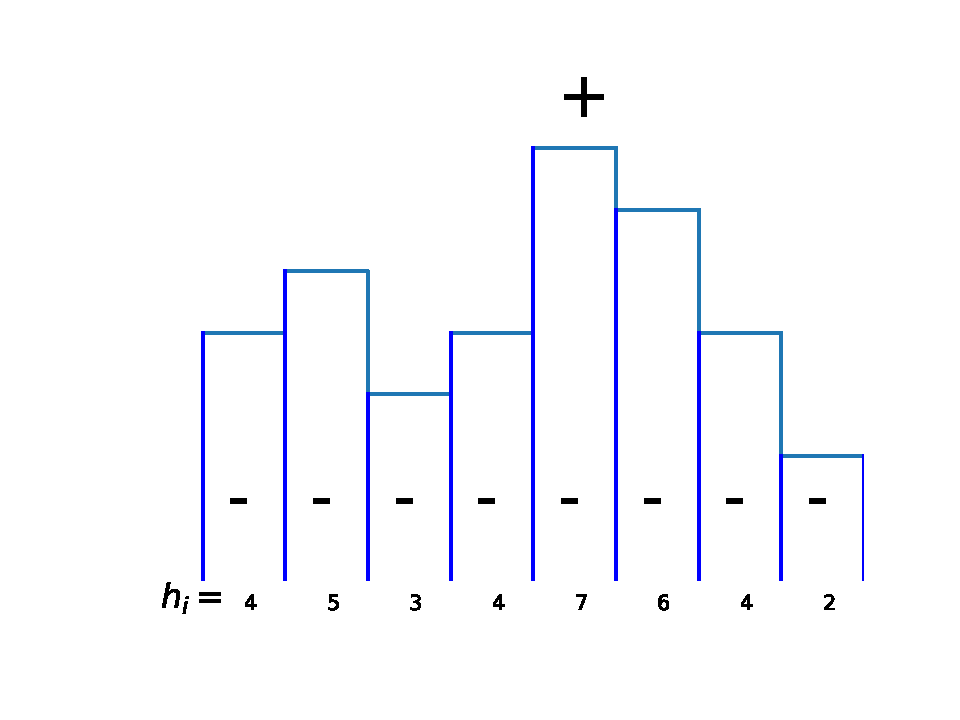
\includegraphics[scale=1]{int-dyn/sos-indiscernable.pdf}
	\caption{Une configuration possible de modèle SOS. Dans la i-ème colonne le bord horizontal de l'interface passe à la hauteur $h_i$. Toutes les particules au-dessus de l'interface sont des spins positifs, et négatifs en dessous. La représentation classique du modèle SOS diffère de ce schéma par l'hypothèse que les particules sont discernables (voir Chapitre \ref{chap-pop}).
	{\color{red} David : pourquoi tu veux mettre cette figure dans un autre chapitre ??}}
    \label{figure-sos}
\end{figure}

En utilisant les identités
\begin{align}
     \min(a,b) &= \frac{|a+b| - |a-b|}{2} \\
    \max(a,b) &=    \frac{|a+b| + |a-b|}{2}
\end{align}
on a
\begin{align}
    \sum_{j=0}^L \sgn(h-j)\sgn(h'-j) = L - 2 |h-h'|
\end{align}
Pour un système d'Ising en deux dimensions de taille $L'\times L$, l'Hamiltonien du modèle d'Ising \ref{hamil-ising}, se réécrit comme 
\begin{align}
    H = 2 J L' (1-L) +2 J \sum_{i=0}^{L'} |h_i-h_{i+1}| + \sum_{i=0}^{L'} V(h_i)
    \label{energie-sos-ising}
\end{align}
où la somme se fait maintenant sur les sites $i$ de hauteur $h_i$ (voir figure \ref{figure-sos}), et le résultat a été divisé par deux pour ne pas compter deux fois les mêmes liens, et 
\begin{align}
    V(h_i) = \sum_{j=0}^L V(\sgn(h-j))
\end{align}
On pose $h_{L'}=h_0$ comme conditions périodiques aux bords.
On peut également calculer directement l'énergie d'un tel système depuis une configuration Solid-On-Solid. Il existe $ L_Y$ liens verticaux par colonne, dont tous sauf un ont une énergie de $-J$, et le lien passant à travers l'interface ayant une énergie de $+J$. L'énergie totale des liens verticaux est donc de $E_y = - J L_X ( L_Y-2)$. De même pour les liens horizontaux, il existe $L_X \times L_Y$ liens au total, dont $\sum_i |h_i-h_{i+1}|$ liens d'énergie $+J$, ce qui nous donne une énergie d'interaction horizontale de $E_x = - J L_X L_Y + 2 \sum_i |h_i-h_{i+1}|$. La somme des deux énergies redonne \ref{energie-sos-ising}.

Le terme $|h_i-h_{i+1}|$ représente la surface de contact horizontale entre les deux phases qui dépend directement de la hauteur, tandis que le terme constant représente la surface de contact verticale.
En simplifiant $2 J = J$ et en retirant l'énergie de volume qui est constante, nous obtenons l'hamiltonien du \textbf{modèle Solid-On-Solid} (SOS)
\begin{align}
    H = J \sum_{i=0}^{L'} |h_i-h_{i+1}| + \frac{V(h_i)+V(h_{i+1})}{2}
    \label{hamil-sos}
\end{align}
où l'on a symmétrisé le potentiel $V(h)$.
Dans le langage liquide/gaz utilisé précédement dans le modèle d'Ising, on peut interpréter la hauteur $h_i$ comme étant le nombre de particules au site $i$, avec les sites au-dessus de l'interface étant considérés comme vides. Lorsque le site $i$ augmente d'une unité, on peut considérer qu'une particule s'est ajoutée au système, et qu'elle s'est évaporée si $h_i$ décroit d'une unité. 

La croissance des cristaux a été le premier système sur lequel le modèle SOS a été développé en 1972 \cite{gilmer_simulation_1972}. Depuis, le modèle a été utilisé pour des systèmes de croissances de cristaux \cite{elwenspoek_kinetic_1987}, a été trouvé en accord avec les expériences de croissance épitaxiale \cite{wilby_scaling_1992}, ou dans le cas des membranes de polymères \cite{gompper_steric_1989}.

Dans le modèle SOS, les $h_i$ peuvent prendre n'importe quelle valeur en tre $0$ et $L$. Une variante de ce modèle est celui où la hauteur $h_{i+1}$ est restreinte uniquement aux valeurs comprises dans $[h_i-a,h_i+a]$. La version du modèle où $a=1$ est appelé le modèle Solid-On-Solid Restreint (RSOS)\cite{privman_transfer-matrix_1989}. Ce modèle est une approximation du modèle SOS à très basse température.  Dans ces conditions, l'interface est très lisse puisque l'on contraint les modes excités de l'interface \cite{kim_conserved_1994,vaysburd_critical_1995}. 

Un modèle qui est plus proche des modèles continus comme l'Hamiltonien \ref{heff} possède une l'interaction gaussienne
\begin{align}
    H = J \sum_{i=0}^{L'} (h_i-h_{i+1})^2 + \frac{V(h_i)+V(h_{i+1})}{2}
    \label{hamil-gsos}
\end{align}
qui possède également une versione restreinte. Le modèle SOS possède, quelque soit l'exposant de l'interaction, une relation étroite avec le modèle $XY$ \cite{knops_exact_1977}.

La dimensionalité du système a été réduite en ne prenant en compte que la hauteur $h_i$ au site $i$ à la place de la position de toutes les particules. L'approximation du modèle SOS implique que les configurations sont analogues à celles d'un mouvement brownien partiellement dirigé auto-évitant. Cette analogie a permis de diagonaliser complètement la fonction de partition dans le cas où il existe un champ magnétique et un potentiel confinant l'interface (nous y reviendrons au paragraphe \ref{par-stab}) \cite{owczarek_exact_1993} et d'étudier les statistiques des déviations extrêmes de l'interface \cite{majumdar_airy_2005,schehr_universal_2006}.


Dans l'ensemble grand-canonique, le nombre de particules dans le système varie, dépendant du potentiel chimique vis-à-vis du réservoir dans lequel il est inséré, ce qui permet à l'interface de bouger librement. Lorsque l'on se place dans l'ensemble canonique, le nombre de particules $N$ sous l'interface est fixe, ce qui introduit une contrainte dans la fonction de partition
\begin{align}
	 Z(N) = \sum_{h_0 h_1 ... h_{L'}} \exp(- \beta \sum_{i} H(h_i,h_{i+1}))  \delta_{\sum_i h_i, N}
	 \label{hamil-sos-cano}
\end{align}
La position moyenne de l'interface est maintenant imposée, ce qui interdit certains microétats, et change les propriétés thermodynamiques de la matrice de transfert comme la distribution des hauteurs de l'interface \cite{siegert_scaling_1993}, même si la moyenne reste la même. Malheureusement, il est impossible de réécrire la contrainte dans le langage des matrices de transfert, empêchant ainsi de calculer analytiquement les différences entre les deux ensembles pour une taille donnée. Il est possible de construire la fonction de partition \textit{ab initio}, mais le grand nombre de sites et de hauteurs permises dans un système classique empêchent le calcul dans un temps CPU raisonnable. 

La fonction de partition \ref{hamil-sos-cano} est en relation vis-à-vis de l'ensemble grand-canonique grâce  au potentiel chimique $\mu$ par
\begin{align}
	 \Xi(\mu) = \sum_N Z(N) \exp((\beta \mu N)
\end{align}
La grande fonction de partition peut s'écrire comme
\begin{align}
    \Xi = \sum_{h_0 h_1 ... h_{L'}}  \exp(-\beta H_{eff}(h_0,h_1,...,h_{L'})
\end{align}
où 
\begin{align}
    H_{eff} = J \sum_{i=0}^{L'} |h_i-h_{i+1}|+ \sum_{i=0}^{L'} V(h_i)-\mu h_i
\end{align}
et de matrice de transfert
\begin{align}
    T(h,h') = \exp\left(-\beta (J |h-h'| - \mu \frac{h+h'}{2} + \frac{V(h)+V(h')}{2} \right)
    \label{tm-sos-grand-cano}
\end{align}

Dans la figure \ref{hauteur-mu}, on montre le nombre moyen de particules par site en fonction du potentiel chimique, pour différentes hauteurs maximales $L$. Ce potentiel chimique simule une pression externe imposée, qui peut soit confiner l'interface vers $h=0$ si $\mu \less 0$ (comme sur la figure), ou le confiner vers $h=L$ si $\mu \greater 0$. 
Ainsi, l'équivalence des ensembles canonique et grand-canonique dans la limite thermodynamique à $\mu$ fixé n'est valable que lorsque le nombre de particules du système canonique $N$ est égal au nombre de particules dans l'ensemble grand-canonique.
\begin{figure}
    \centering
	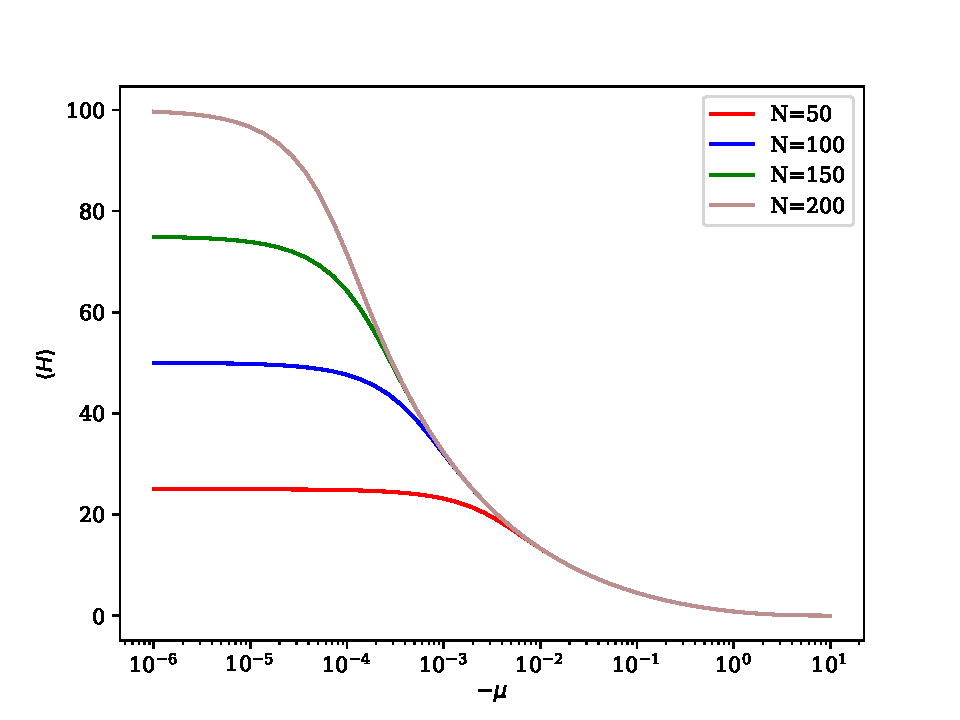
\includegraphics[width=0.7\linewidth]{int-dyn/hauteur-tm-sos.pdf}
	\caption{Position d'équilibre de l'interface \ref{tm-sos-grand-cano} en fonction de $- \mu$ via diagonalisation de la matrice de transfert \ref{tm-sos-grand-cano}. Lorsque le potentiel chimique est trop faible, l'interface est délocalisée et se retrouve à la position $\frac{N}{2}$. }
	\label{hauteur-mu}
\end{figure}

Comme dans le modèle d'Ising, il existe une bijection entre l'usage d'un champ magnétique conjugé à une aimantation par site et l'usage d'un potentiel chimique conjugué à une densité de particules. Nous parlerons donc sans ambigüité de potentiel chimique pour tout potentiel $V(h_i)$ que nous étudierons plus tard, ainsi que de densité de particules $M$.


Note that the case where $V(h)=P_0h$ simulates the SOS with and externally imposed pressure. This model is also equivalent mathematically to the SOS model in a grand canonical ensemble, where we think of the height as representing a number $h_i$ of particles stacked at each site $i$ and $P_0=-\mu$ where $\mu$ is the chemical potential (which can be positive or negative). However this is not strictly true, if we consider the case where $\sigma=0$ then in the SOS the configuration where all the particles are concentrated at a single site is equally as probable as that where all sites have the same number of particles and physical intuition tells us that the latter configuration should be more probable.

%%%%%%%%%%%%%%%%%%%%%%%%%%%%%%%%%%%%%%%
  \subsection{Matrice de Transfert}
%%%%%%%%%%%%%%%%%%%%%%%%%%%%%%%%%%%%%%%

	De manière plus générale, l'Hamiltonien d'un système avec des interactions entre les particules peut se réécrire comme $H = \sum_{< ij >} H(h_i,h_j)$ avec
\begin{align*}
  H = \sum_{i=0}^{L'} f(h_i,h_{i+1}) + V(h_i,h_{i+1}) 
\end{align*}
où $f(h_i,h_j)$ est l'énergie d'interaction entre plus proches voisins et $V(h_i,h_j)=\frac{V(h_i)+V(h_j)}{2}$ le potentiel symmétrisé. Pour un système possédant $L'$ sites pouvant continr des valeurs dans $[0,L]$, la fonction de partition de notre système s'écrit 

\begin{align}
 Z = \sum_{h_1=0}^{L} \sum_{h_2=0}^{L}... \sum_{h_{L'}=0}^{L¡} \exp(- \beta \sum_{i=0}^{L'} H(h_i,h_{i+1}))
   = \sum_{h_1 h_2 ... h_{L'}} \prod_{i=_0}^{L'} \exp(-\beta H(h_i,h_{i+1}))
\end{align}

La matrice 
\begin{align}
    T(h_i,h_j) = e^{-\beta H(h_i,h_j)}
    \label{matric-transfert}
\end{align}
est appelée matrice de transfert. On a représenté dans la figure \ref{mat-inf} une matrice infinie correspond à la limite thermodynamique dans le cas où les sites peuvent prendre n'importe quelle valeur dans $[-\infty,\infty]$, qui correspond au cas où l'interface est centrée en $h=0$ et ne possède pas de conditions aux bords. Lorsqu'il s'agit de diagonaliser cette matrice infine numériquement, il suffit de faire la translation $h_i \to h_i - \frac{L}{2}$, où $L$ est la taille de la matrice de transfert, tendant vers l'infini.

Puisque le système est périodique (c'est-à-dire que $h_{L+1} = h_1$),  la matrice est périodique également, c'est-à-dire que $T(h_L,h_{L+1}) = T(h_L,h_1)$ \cite{pearce_exact_1989}, et elle est également symétrique, La matrice de transfert peut donc être diagonalisée, nous écrivons ses vecteurs valeurs propres comme
\begin{align}
    T | \lambda> = \lambda |\lambda>
\end{align}
Ces vecteurs propres sont également orthonormaux 
\begin{align}
    < \lambda | \lambda'> = \delta_{\lambda \lambda'}
\end{align}
On note par $\lambda_0$ la plus grande valeur propre de T, par $\lambda_1$ la deuxième plus grande valeur propre etainsi de suite. 
Ainsi on peut diagonaliser la fonction de partition par la trace de la matrice de transfert \cite{abraham_transfer_1973}
\begin{align}
  Z = \sum_{h_1 h_2 ... h_{L'}} \prod_{i} T(h_i,h_{i+i}) = Tr( T^{L'})  = \sum_\lambda <\lambda | T^{L'} | \lambda> = \sum_\lambda \lambda^{L'}
  \label{partition-trace-lambda}
\end{align}

\begin{figure}
    \begin{align}
    T = \begin{bmatrix} 
            \ddots & \vdots & \reflectbox{$\ddots$} \\ 
            e^{-\beta H(-1,-1)} &  e^{-\beta H(-1,0)} & e^{-\beta H(1,-1)} \\
            \dots & e^{-\beta H(0,0)} & \dots  \\
            e^{-\beta H(1,-1)} & e^{-\beta H(1,0)} & e^{-\beta H(1,1)}   \\ 
             \reflectbox{$\ddots$} & \vdots &\ddots  \\ 
        \end{bmatrix}
    \end{align}
    \caption{Matrice de transfert infinie et symmétrique \ref{matric-transfert}.}
    \label{mat-inf}
\end{figure}

Dans la limite thermodynamique $L' \to \infty$, seul le plus grand vecteur propre est relevant, puisque la fonction de partition devient
\begin{align}
    Z(L\to \infty) \simeq \lambda_0^{L'}
\end{align}
Nous trouvons alors que l'énergie libre par site est égale à 
\begin{align}
	F =  - \frac{1}{L' \beta} \ln(Z) \simeq - \frac{1}{\beta } \ln( \lambda_0)
	\label{energie-libre-site}
\end{align}
Dans la figure \ref{fig-thermo-libre} on montre l'évolution de l'énergie libre par site $F(L')$ dans le cas d'un potentiel nul.On détermine alors que l'approximation de la limite thermodynamique est vraie pour $L' \greater 150 $.
\begin{figure}
    \centering
	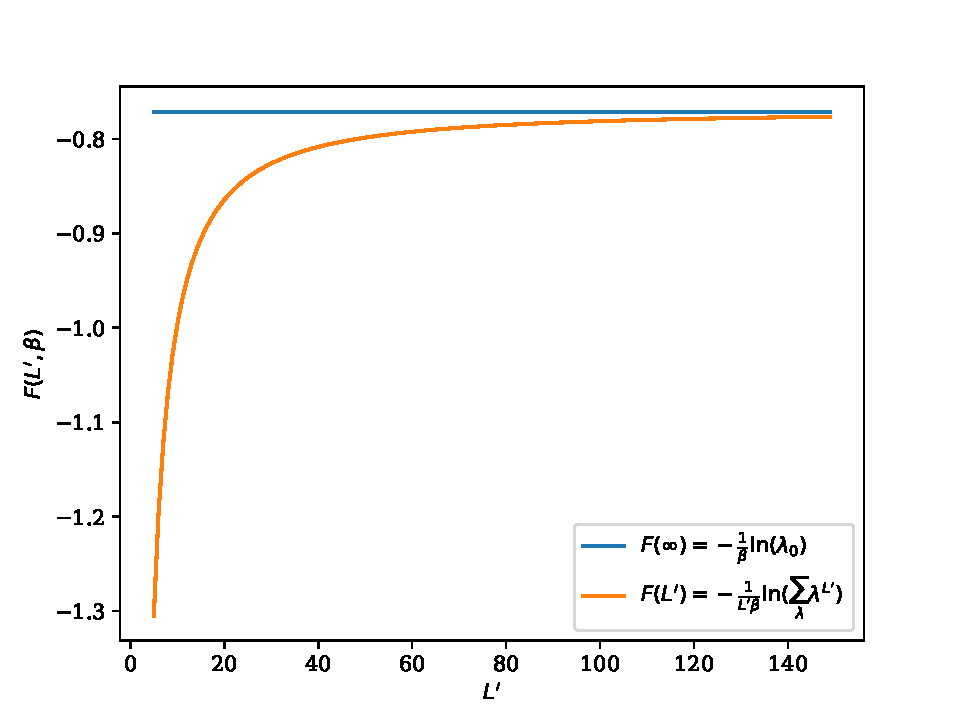
\includegraphics[width=0.7\linewidth]{int-dyn/freeene-thermo-libre.pdf}
	\caption{Énergie libre par site $F(L')$ en fonction du nombre de sites $L'$ comparé à la limite thermodynamique $F(\infty)$, pour un système de hauteur $L=100$, $\beta=1$, $J=1$ et $V(h_i)=0$.}
	\label{fig-thermo-libre}
	\vspace{-0.5cm}
\end{figure}  
Afin de calculer la densité moyenne par site $M$, on introduit la matrice des hauteurs $\hat{M}$ définie par son action sur les vecteurs $|h>$ de la base de la matrice de transfert par
\begin{align}
    <h|\hat{M} |h'> = \delta_{h,h'} h
\end{align}
On trouve alors la densité par site 
\begin{align}
	M = < h > = \frac{1}{L'} \sum_i h_i =  \frac{1}{Z} \sum_\lambda \lambda^{L'} < \lambda | \hat{M} | \lambda > \simeq < \lambda_0 | \hat{M} | \lambda_0 > 
	\label{tm-magnetisation}
\end{align}
On en déduit la variance sur la hauteur par site
\begin{align}
	w^2 = < (h - M)^2 > = \frac{1}{Z} \sum_\lambda \lambda^{L'} < \lambda | \hat{M}^2 | \lambda > - < \lambda | \hat{M}| \lambda >^2  \simeq  < \lambda_0 | \hat{M}^2 | \lambda_0 > - M^2
\end{align}
On peut retrouver ces deux observables en calculant le premier et le second moment de la densité de probabilité qu'un site se trouve à la hauteur $h$
\begin{align}
	p(h) = \frac{1}{Z} \sum_\lambda \lambda^{L'} <\lambda | h >^2 \simeq < \lambda_0 | h >^2
\end{align}
La fonction de corrélation à deux points du système se calcule grâce à la formule
\begin{align}
    C(r) &= < h_i h_{i+r} > - M^2 = \frac{1}{Z} \sum_{\lambda \neq \lambda_0} < \lambda_0 | M | \lambda > < \lambda | M | \lambda_0 > \left( \frac{\lambda}{\lambda_0} \right)^r  
\end{align}
qui devient, dans la limite où $r$ est grand, 
\begin{align}
    C(r) \simeq < \lambda_0 | M | \lambda_1 > < \lambda_1 | M | \lambda_0 > \left( \frac{\lambda_1}{\lambda_0} \right)^r
\end{align}
{\color{red} what did you mean in your corrections by "explain when this is true-what happens to $\lambda_2$ etc" ? }
À grande distance, cette fonciton de corrélation a un charactère exponentiel, ce qui nous permet de définir la longueur de corrélation à grande distance $\xi$
\begin{align}
    \xi = - \frac{1}{\ln(\frac{\lambda_1}{\lambda_0})}
    \label{longueur-correl-thermo}
\end{align}

%
%%%%%%%%%%%%%%%%%%%%%%%%%%%%%%%%%%%%%%
%	\subsection{États libres dans un système SOS infini}
%	\label{par-stab}
%%%%%%%%%%%%%%%%%%%%%%%%%%%%%%%%%%%%%%
%
%Prenons un système de taille $L$ dans la limite thermodynamique $L'\to \infty$. Comme vu précédement, seules les valeurs de la plus grand valeur propre influe sur les propriétés statistiques. Soit 
%\begin{align}
%    \psi_\lambda(h)= <h|\lambda>
%\end{align}
%la projection du vecteur propre associé à la valeur propre $\lambda$ de la matrice de transfert sur la base des hauteurs $|h>$ dans un système infini de part et d'autre de l'interface.
%Dans la limite $\beta=0$, c'est-à-dire pour une température infinie, tous les termes de la matrice de transfert sont égaux à $1$, menant à des vecteurs propres nuls. Dans ce cas, la densité de probabilité $p(h)$ est nulle pour tout $h$, ce qui signifie qu'il n'existe pas d'interface. Le modèle SOS n'est donc pas valable dans cette limite. De même, pour une température nulle $\beta=\infty$, la matrice de transfert devient la matrice identité. Les valeurs propres deviennent toutes égales à $1$ et les vecteurs propres sont $\psi_i(h) = \delta_{h,i}$ où ici $i$ est l'indice de la i-ème valeur propre $\lambda_i = 1$. La probabilité de trouver l'interface à la hauteur $h$ devient $p(h) = \frac{1}{Z}\sum_{i} <\lambda_i | h >^2 = 1$. La température nulle a pour effet de geler l'interface sur une seule hauteur, même si toutes les hauteurs sont équiprobables. Bien que les micro-états soient extrêmement différents pour une température finie, les propriétés macroscopiques sont identiques à cause du même poids statistique associé à chaque état.
%
%Pour une température finie et en absence de potentiel\cite{guyer_sine-gordon_1979,chui_pinning_1981}, l'équation du vecteur propre donne
%\begin{align}
%	\sum_{h=-\infty}^\infty T(h,h') \psi_\lambda(h) = \lambda \psi_\lambda(h')
%\end{align}
%En introduisant l'ansatz $\psi_\lambda(h) = \alpha_{\lambda}^h$ et en séparant de la somme les termes pour $h$ négatifs et positifs, on trouve aisément que 
%\begin{align}
%	\lambda = \frac{\sinh(\beta J)}{\cosh(\beta J)-(\alpha_{\lambda}+\alpha_{\lambda}^{-1})} 
%\end{align}
%Dans la limite thermodynamique, la probabilité de présence de l'interface à la hauteur $h$ est $p(h) = <\lambda_0|h>^2 = |\psi_0(h)|^2$. Le système ne possédant aucune brisure de symétrie particulière, la probabilité $p(h)$ est finie pour tout $h$ avec $p(h)=p(-h)$. Dès lors, l'ansatz supposé $\psi_\lambda(h) = \alpha_{\lambda}^h$ implique que $\alpha_{\lambda}$ soit de la forme $e^{ik}$ où $k$ est la longueur d'onde associée à la valeur propre $\lambda$. On obtient que 
%\begin{align}
%	\psi_k(h) =& e^{ikh} \\
%	\lambda =& \frac{\sinh(\beta J)}{\cosh(\beta J) - \cos(k)}
%	\label{lambda-sos}
%\end{align}
%
%L'existence d'une solution de ce genre indique que l'interface n'est pas localisée dans le cas d'un système infini (ou semi-infini) en absence de tout potentiel, ce qui conduit à de nombreux problèmes numériques. 
%
%Une manière simple de localiser l'interface est de rajouter un potentiel $V(h) = -B \delta_{h,0}$ \cite{chui_pinning_1999,chalker_pinning_1981,chalker_pinning_1982}, qui augmente la probabilité de présence de l'interface à $h=0$. La recherche d'un état localisé nous donne un ansatz de la forme 
%\begin{align}
%	\psi_\lambda(h) = \begin{cases} |\alpha|^h & \text{si } h \neq 0 \\ \psi_{\lambda,0} & \text{sinon} \end{cases} 
%\end{align}
%L'équation du vecteur propre devient
%\begin{align}
%	\sum_{h=-\infty}^\infty \exp(\beta |h-h'|- \beta B \delta_{h,0}) \psi_\lambda(h) = \lambda \psi_\lambda(h')
%\end{align}
%En notant $T(h,h') = R^{|h-h'|}$ pour $h \neq h' \neq 0$,  on obtient la même équation à un signe près dans l'exposant que l'on soit à $h'\greater 0$ ou $h' \greater 0$
%\begin{align}
%	\left( \frac{R}{\alpha} \right)^{\pm h'} \left[ \psi_{\lambda,0} + \frac{R \alpha}{1 - R \alpha} + \frac{\alpha}{R - \alpha} \right] + \left[ \frac{1}{1-R \alpha} - \frac{R}{R-\alpha} \right] = \lambda
%\end{align}
%Puisque cette équation est vraie pour tout $h'$, le premier terme doit être nul, ce qui nous donne
%\begin{align}
%	\psi_{\lambda,0} &= - \frac{\alpha}{R-\alpha}-\frac{R \alpha}{1-R \alpha} \\
%	\lambda &= \frac{1}{1-R \alpha} - \frac{R}{R-\alpha}
%\end{align}
%L'équation du vecteur propre à $h'=0$ nous donne par ailleurs 
%\begin{align}
%	\psi_{\lambda,0} + 2 \frac{R \alpha}{1-R \alpha} = \lambda \psi_{\lambda,0} e^{-\beta B}
%\end{align}
%L'existence d'une solution cohérente $\alpha \less 1$ autorise la présence d'une interface localisée grâce à un potentiel dit d'épinglage (\textit{pinning}) \cite{burkhardt_localisation-delocalisation_1981,kroll_solid--solid_1981,kroll_pinning_1982,kroll_interface_1983}.
%Dans le cas d'une géométrie semi-infinie, la présence d'un potentiel chimique exerçant une pression sur l'interface permet de la maintenir confinée, comme expliqué dans la section \ref{subsec-c-gc}.
%
%D'autres méthodes existent pour confiner l'interface. Le cisaillement d'une interface diminue sa largeur et permet de la localiser dans l'espace. On peut également proposer deux potentiels chimiques différents pour chaque phase à une hauteur de l'interface prédéfinie, comme le ferait un laser dans un liquie binaire dont chaque phase  a un incident de réfraction différent \cite{casner_laser-induced_2003,delville_laser_2009} (voir chapitre \ref{sec_laser}). Dans un système infini, une autre possibilité est de définir un champ magnétique symétrique rendant plus difficile la présence de l'interface loin de $0$. 


%%%%%%%%%%%%%%%%%%%%
    \section{Conclusion}
%%%%%%%%%%%%%%%%%%%%    
